\section{Extracting railway network data}
Nowadays, most passenger train companies provide online platforms on which people can buy train tickets. These platforms usually contain sufficient data to reconstruct some form of the railway network:
\begin{itemize}
    \item train numbers,
    \item station names.
    \item train routes between stations.
    \item travel time from one station to the next.
    \item network delays and failures.
\end{itemize}

One important piece of data that is \emph{not} available to the public is the physical track layout and throughput.
This means that, if one were to use data from this source, the resulting network would be made up of \emph{train routes}, rather than actual \emph{railways}. Even if some results will be similar, one must not forget that the two are very distinct entities.
Train routes are managed by different companies; they can vary quiclky in time due to demand and cost requirements. Railways, on the other hand, are physical structures that cannot be altered, unless a significant investment of time and money is made.

\subsection{Trainline}
\emph{Trainline} is a UK-based train-ticket company. They define themselves as: \blockquote{We are Europe’s leading train and coach app. To put it simply, we are a one-stop-shop for train and coach travel. Every day, we gather routes, prices, and travel times from over 270 rail and coach operators in 40 countries, so that everyone can buy tickets quickly and save time, effort, and money.\footnote{\url{https://www.thetrainline.com/about-us}}}
What their company does, in essence, is gather all the data from the major European train companies and then sell it. 
As a matter of fact, when a person buys a ticket through their platform, a small commision gets paid to Trainline, as an exchange for the ticket availability data\footnote{\url{https://www.trainlinegroup.com/what-we-do/business-model/}}.
The sale of the data can also happen at a larger scale, through their private-access \emph{Global Travel API}\footnote{\url{https://www.thetrainline.com/solutions/api}}. 

\subsection{Scraping the data}
\subsubsection{Legal Issues}
I was not able to obtain access to the Trainline API, and thus I had to manually scrape their data from their website. This came with the advantage that it was completely free, but with the drawback that it is a legal gray area. Although at the moment of writing their Terms of Service\footnote{\url{https://web.archive.org/web/20240716112036/https://www.thetrainline.com/terms}} do not appear to explicitly prohibit scraping, I consider the study I made in the following sections to be valid only for my personal use (that is, for the purpose of taking the Complex Networks exam).

\subsubsection{The scraping process}
Trainline offers a portal that contains a list of all of the stations reached by their routes\footnote{\url{https://www.thetrainline.com/en/stations}}.
From this webpage, it is possible to extract a list containing the URL for each station page by looking at its source code. Once we have this list, we can start downloading each page individually.
From every station page we can then extract the information of the most relevant destinations that can be reached from that station.
This whole process is described in detail in \autoref{fig:scraping-process}.

\begin{figure}
    \centering
    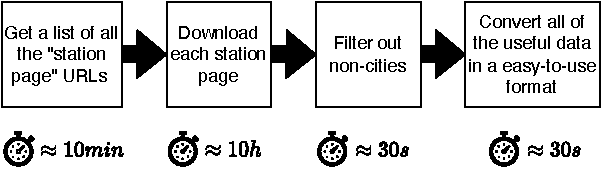
\includegraphics[width=1\linewidth]{report//assets/data-scraping.pdf}
    \cprotect\caption{Overview of the scraping process. The first step is getting a list of URLs for all of the train stations. This is done by hand, by analyzing the code of the \verb|/en/stations| page. The code contains one JavaScript array with the list of all URLs. With JavaScript it is easy to download each page programmatically. The maximum speed I was able to achieve was $\approx 20pages/s$, but that would trigger the CloudFlare DoS protection. In the end I had to let the scraper run overnight, with a speed of about one page every two seconds. The last step is just a matter of runinng through each HTML file with a RegExp that filters out all the needed data. This is pretty straighforward, as all the data is contained inside a JavaScript object which can be easily parsed. The third step is explained in the following section (\ref{subsubsec:data-in-numbers}).}
    \label{fig:scraping-process}
\end{figure}


\subsubsection{Data in numbers}
\label{subsubsec:data-in-numbers}
Before moving on, I want to point out again one subtlety in the data that I got. That is, Trainline offers information on two types of "station". Some are the \emph{real}, physical stations and some other are \emph{fictional aggregates} (which I will call \emph{cities}) of some number of real stations, usually found withing the same city.
This aggregate is generated by Trainline using some unknown algorithm. Even though I trust that this data is accurate, it might be difficult to track its source outside of Trainline.
For my study, I constructed the network using only the fictional aggregates.


Now, let us have a brief look at the data I got. 
In total, I have downloaded $18,502$ webpages ($4.95GB$ of data). Out of these, $248$ were cities. The total number of links reported between the cities was $1976$.


\subsection{Building the adjacency matrix}
Each station on the Trainline website has a list of the most common stations that can be reached starting from it. With this piece of information, it is easy to construct a (directed) adjacency matrix $A$. Moreover, the data contains the average number of trains per day that reach said destinations, and the average time it takes to get there. We can use this information to construct a rate matrix $W$ by multiplying each link by the ratio
\begin{equation*}
    \frac{\text{Number of daily trains through one route}}{\text{Average time it takes to complete the route}}.
\end{equation*}
The resulting matrix is plotted in \autoref{fig:asymm-plot-full} and a zoomed in, cropped version of it is plotted in \autoref{fig:asymm-plot-half}. The rows and columns have been sorted in order of population of the respective cities.
I find it nice to have a clear, human-readable plot of the (unweighted) data, and I provided it in \autoref{fig:big-plot}.

\begin{figure}[h]
    \centering
    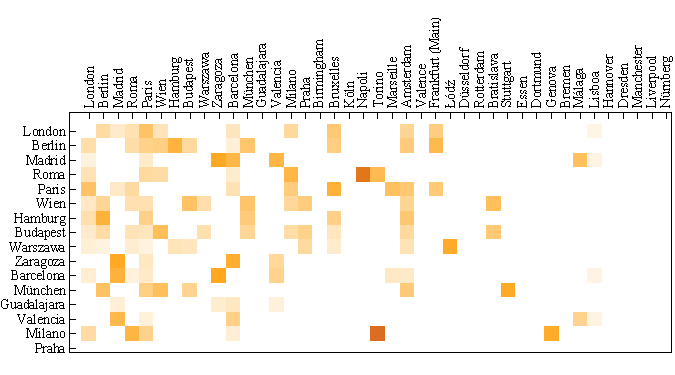
\includegraphics[width=\linewidth]{assets/asymmPlotHalf.pdf}
    \caption{
    Detail of the adjacency matrix of the European train network, sorted by city population. Dense connections are evident among major hubs (left side of the matrix), indicating high connectivity, but they decrease with smaller cities.}
    \label{fig:asymm-plot-half}
\end{figure}

The resulting matrix shows a gradient from left to right. This is a consequence of the fact that the Trainline data shows only the most common routes that start in any one city. It follows that
\begin{enumerate}
    \item smaller cities will often display link information to bigger cities (like country or state Capitals), and
    \item bigger cities will often display link information between themselves.
\end{enumerate}
In the zoomed-in graph of \autoref{fig:asymm-plot-half} it is easy to see this phenomenon: most links to the left of the matrix (where the big capital cities are) are two-ways and the matrix gets sparser and sparser the more we look to the right. 
This phenomenon indicates bias in the data, but it can easily corrected by making the assumption that \emph{every train that leaves a destination must come back to it}. We can then make the rate matrix symmetric by mirroring it across the diagonal\footnotemark. The resulting matrix is plotted in \autoref{fig:symm-plot}. 

\footnotetext{If a cell $W_{nm}$ is empty, and the transposed cell $W_{mn}$ is not, we set $W_{nm} = W_{mn}$. If both cells contain a value, we set each one of them to the average: $W_{nm} = W_{mn} = \frac 1 2 (W_{nm} + W_{mn})$.}

